% -*- Index -*-


\chapter{Strategies}
\label{chap:Strategies}

\index{strategy|(}

\IceT contains several parallel image compositing algorithms.  The type of
compositing algorithm to use is selected by choosing a
\index{strategy}\keyterm{strategy}.  This chapter describes the underlying
algorithm of each strategy.  This user's guide will give qualitative
comparisons between the strategies, but for a more quantitative analysis,
see the following paper.

\begin{quote}
  Kenneth Moreland, Brian Wylie, and Constantine Pavlakos.  ``Sort-last
  parallel rendering for viewing extremely large data sets on tile
  displays,'' In \emph{Proceedings of IEEE Symposium on Parallel and
    Large-Data Visualization and Graphics}, October 2001, pp. 85--154.
\end{quote}

A strategy is specified using the \CFunc{icetStrategy} function.

\begin{Table}{3}
  \textC{void }\CFunc{icetStrategy}\textC{(}&\CType{IceTStrategy}&\CArg{strategy}\quad\textC{);}
\end{Table}

The \CArg{strategy} is set to one of the identifiers for the strategies
documented in the following sections of this chapter.  A string documenting
the current strategy can be retrieved with the \CFunc{icetGetStrategyName}
function.

To describe the \IceT compositing algorithms, we will use the example
parallel rendering problem shown in Figure~\ref{fig:ExampleInputs} where 6
processes are each rendering their own piece of a shuttle model to a two
tile display.

\begin{figure}
  \centering
  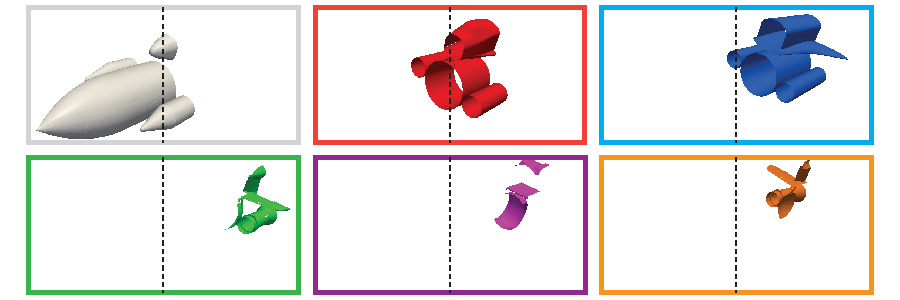
\includegraphics{images/AllInput}
  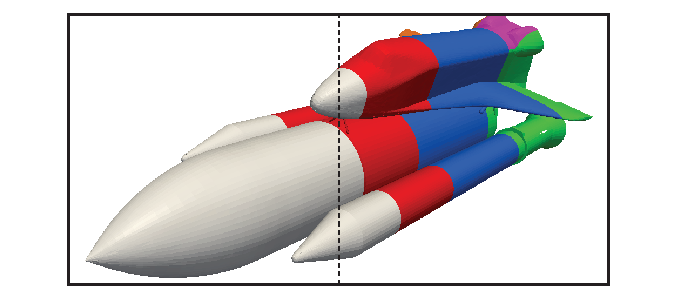
\includegraphics{images/CompositedInput}
  \caption[Example compositing problem.]{An example of six processes
    rendering to two tiles (top) and their composited image (bottom).}
  \label{fig:ExampleInputs}
\end{figure}

In this example, processes are denoted, in no particular order, by the
colors gray, red, blue, green, purple, and orange.  The colors of the
geometry correspond to the process that generated each piece.  Image
boarder colors denote the process that generates and holds that image.
(Apologies to those having troubles resolving the colors due to poor
display or vision deficiencies.  It should not be hard to follow the
descriptions either way.)

\section{Single Image Compositing}

\index{single~image~composite|(}
\index{compositing!single~image|(}

Before discussing the multi-tile image compositing algorithms implemented
by \IceT, we visit the standard single image compositing algorithms.  You
cannot directly select a single image compositing algorithm as a strategy
(most of the multi-tile algorithms work well in ``single-tile'' mode), but
these compositing algorithms are used as ``subroutines'' in some of the
multi-tile algorithms.  A reference to a
\index{single~image~composite~network}\keyterm{single image composite
  network} in the subsequent compositing algorithm descriptions refers to
the algorithms described here.

\subsection{Tree Compositing}

\index{compositing!tree|(}
\index{tree~composite|(}
\index{binary~tree~composite|(}

\IceT internally has two single image composite implementations.  The first
of which is the \keyterm{tree composite} algorithm (sometimes also called
binary tree composite due to its pair-wise grouping).  The basic network
for tree composite is shown in Figure~\ref{fig:BinaryTree}.

\begin{figure}
  \centering
  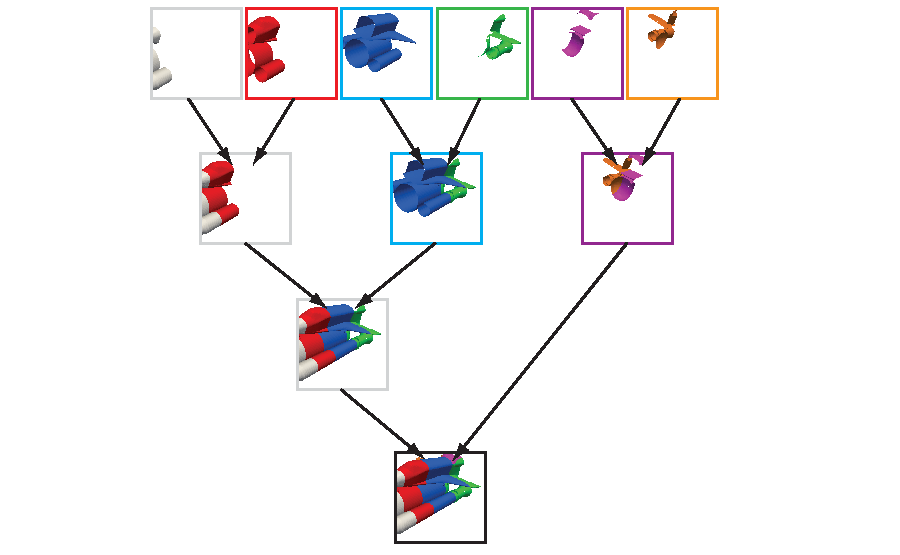
\includegraphics{images/BinaryTree}
  \caption[Tree composite network.]{Tree composite network.  Arrows
    represent the passing of data from one stage to the next.  Processes
    receiving multiple images composite them together.}
  \label{fig:BinaryTree}
\end{figure}

The tree compositing algorithm is organized in stages.  At each stage the
processes pair up.  One of the processes sends its data to its pair and
then drops out of the computation.  The receiving process combines the two
images (using the \index{compositing~operation}compositing operation
described in
Chapter~\ref{sec:Customizing_Compositing:Compositing_Operation}) and
continues to the next stage.  Processing continues until there is only one
image (and one process) remaining.

As just defined, the tree composite algorithm only handles process counts
that are a power of two (that is, the number of processes is equal to $2^i$
for some integer $i$).  \IceT handles non-powers of two gracefully.  At any
stage where the number of processes is not even and one of the processes
cannot be paired, that leftover process does nothing for that stage but
then continues to participate in the next stage.  An example of this can be
seen in the second stage of Figure~\ref{fig:BinaryTree}.

The advantages of tree composite are its regular and efficient data
transfers.  The limiting factor of tree compositing is that at each stage
of the algorithm half of the processes drop out of the computation.  Thus,
for more than a few processes tree compositing provides poor process
utilization.

\index{binary~tree~composite|)}
\index{tree~composite|)}
\index{compositing!tree|)}

\subsection{Binary-Swap Compositing}

\index{compositing!binary~swap|(}
\index{binary~swap~composite|(}

The second single image compositing algorithm used internally by \IceT is
the \keyterm{binary swap} algorithm.  The basic network for binary-swap
composite is shown in Figure~\ref{fig:BinarySwap}

\begin{figure}
  \centering
  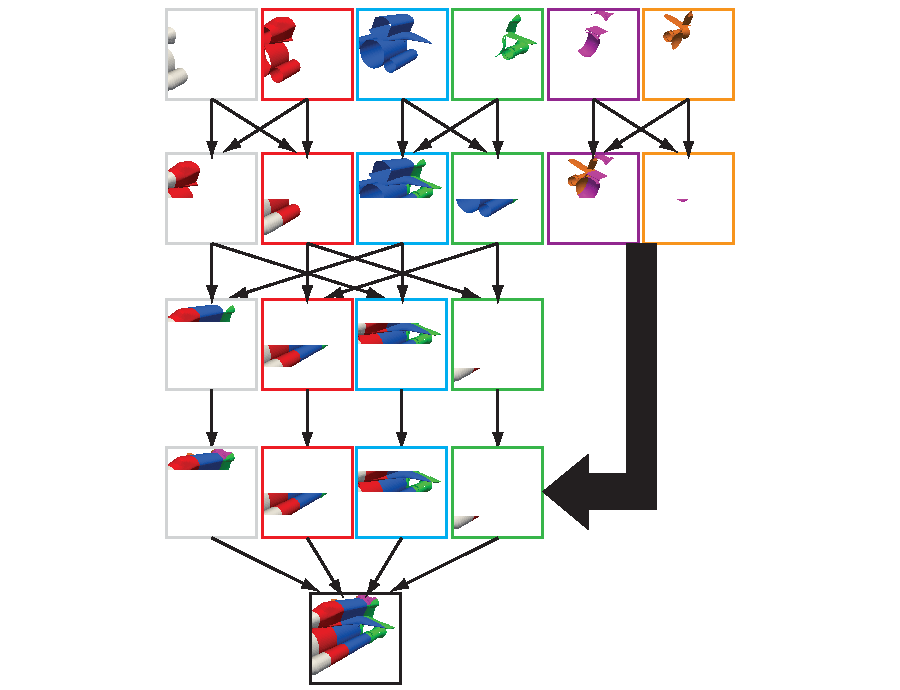
\includegraphics{images/BinarySwap}
  \caption[Binary-swap composite network.]{Binary-swap composite network.
    Arrows represent the passing of data from one stage to the next.
    Processes receiving multiple images composite or stitch them together.
    At most stages each process divides its image data and distributes it.
    The distribution of image data can be inferred from the target images.}
  \label{fig:BinarySwap}
\end{figure}

Like tree compositing, binary swap is organized in stages, and at each
stage the processes pair up.  However, rather than have one process send
all the data to the other, the image space is divided in two and the
processes swap image data so that each process has all the data for part of
the image.  At the next stage, the processes pair up again, but with
different partners that have the same partition of the image.  Processing
continues until each of the $N$ processes have an image $1/N$ the size of
the original image.  At this point, all the processes send their sub-image
to the display processes where the images are stitched together.

As just defined, the binary-swap composite algorithm only handles processes
that are a power of two (that is, the number of processes is equal to $2^i$
for some integer $i$).  Some binary-swap implementations handle non-powers
of two by reducing the problem to the next largest power of two and
dropping the leftover processes, but \IceT handles non-powers of two more
gracefully than that.  Instead, \IceT first finds the largest group of
processes that is a power of two, makes a partition out of them, then finds
the next largest group of processes that remain that is a power of two,
makes a partition out of them, and so on.  Each partition runs binary-swap
independently up to the point where each process has its own piece of data.
At this point, the smaller partitions send their image data to processes of
the larger partitions, dividing up images where necessary.  The largest
partition then finishes the compositing in the normal way by collecting all
of the pieces.

An example of compositing with a non-power of two is given in
Figure~\ref{fig:BinarySwap}.  The six processes are partitioned first into
a group of 4 and then into a group of 2.  After swapping, the processes in
the smaller group send images to the larger group.  In this case, the purple
process sends image data to the gray and blue processes, and the orange
process sends to the red and green processes.

Like tree composite, binary swap exhibits regular and efficient data
transfers.  In addition, binary swap involves the use of all the processes
throughout most of the compositing.  Consequently, binary swap exhibits
very good process utilization and scaling with respect to the number of
processes on which it is run.

The most inefficient part of binary swap is the collection of image
fragments at the end, which is an extra step that tree composite does not
need to take.  Through some empirical studies, we found that the binary
tree algorithm was more efficient than binary swap on less then 8 processes and
less efficient on more than 8 processes.  Consequently, \IceT automatically
switches between the two algorithms based on the amount of processes
involved in the compositing.

\index{binary~swap~composite|)}
\index{compositing!binary~swap|)}

\subsection{Ordered Compositing}

\index{compositing!ordered|(}

In some applications, the order in which images are composited together
makes a difference (see the Volume Rendering section in
Chapter~\ref{sec:Customizing_Compositing:Volume_Rendering}).  The details
on how ordered compositing is achieved is not given here, but the basic
idea for both compositing algorithms is that they first swizzle the
processes so that their order matches the order in which the images need to
be composited together.  When compositing images together, they make sure
to maintain over/under constancy based on the swizzled ranks from the
originating processes.  The networks are also managed such that no two
images are composited that are not directly ``next'' to each other (that
is, there is no image that needs to be inserted between them).

\index{compositing!ordered|)}

\index{compositing!single~image|)}
\index{single~image~composite|)}

\section{Reduce Strategy}
\label{sec:Strategies:Reduce}

\index{strategy!reduce|(}
\index{reduce~strategy|see{strategy, reduce}}

\sticky{Supports ordered compositing.}

\index{strategy!reduce|)}

\section{Split Strategy}
\label{sec:Strategies:Split}

\index{strategy!split|(}
\index{split~strategy|see{strategy, split}}

\sticky{Does not support ordered compositing.}

\index{strategy!split|)}

\section{Virtual Trees Strategy}
\label{sec:Strategies:Vertial_Trees}

\index{strategy!virtual~trees|(}
\index{virtual~trees|see{strategy, virtual trees}}

\sticky{Does not support ordered compositing.}

\index{strategy!virtual~trees|)}

\section{Serial Strategy}
\label{sec:Strategies:Serial}

\index{strategy!serial|(}
\index{serial~strategy|see{strategy, serial}}

\sticky{Supports serial strategy.}

\index{strategy!serial|)}

\section{Direct Strategy}
\label{sec:Strategies:Direct}

\index{strategy!direct|(}
\index{direct~strategy|see{strategy, direct}}

\sticky{Supports serial strategy.}

\index{strategy!direct|)}

\section{Implementing New Strategies}

\index{strategy|)}
